\chapter{How does X Influence Novelty, Complexity, and Adaptation?}
\label{ch:influencing-cna}

\noindent
% Authors: Matthew Andres Moreno, Santiago Rodriguez Papa, and Charles Ofria \\
This chapter is in proposal.

\section{Event-driven vs. Sensor-driven Genetic Encoding}

SignalGP is a biologically-inspired approach that allows digital organisms to dynamically respond to environmental signals.
Each event (i.e., a signal from the environment or other agent) is associated with a tag to identify it; modules in the digital organism will be triggered to execute when an event with a matching tag occurs (Figure \ref{fig:signalgp-schematic;ch:influencing-cma}) \citep{lalejini2018evolving}.

We have shown that SignalGP allows evolved programs to engage in a broad range of environmental interactions and can better incorporate context into their behaviors.
Lalejini et. al. found that tag-based genetic regulation dramatically improved the solution success rate on sensor-intensive and context-dependent problems \citep{lalejini2018evolving, lalejini2021tag}.
Despite these positive results, this methodology has not yet been directly examined in an artificial life context, especially for its capacity to produce biologically realistic interactions.
Our goal is to enrich the toolbox of artificial life researchers to conduct evolution experiments while also expanding the applications to genetic programming.

\begin{figure}[h]

\centering
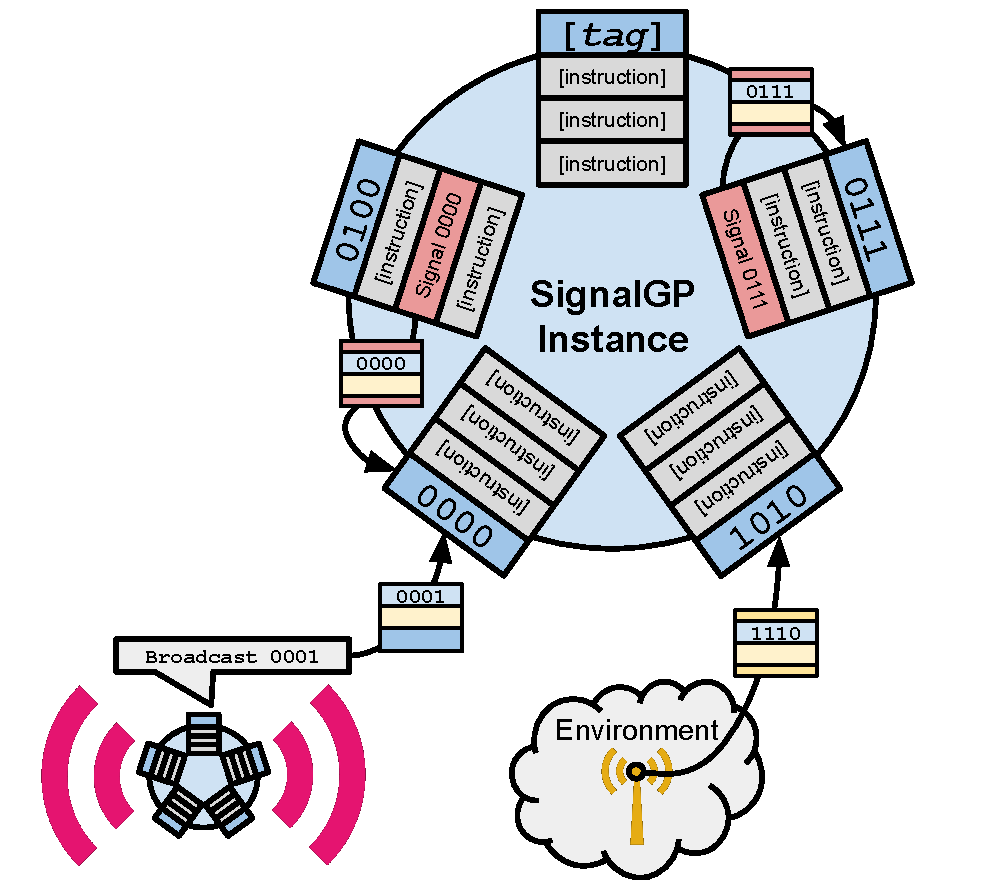
\includegraphics[width=0.5\textwidth]{img/signalgp-schematic}

\caption{SignalGP schematic depicting interactions between an agent and its environment}
\label{fig:signalgp-schematic;ch:influencing-cna}

\end{figure}


DISHTINY is a digital framework designed to study open-ended transitions to multicellularity \citep{moreno2019toward}.
In preliminary studies, we have used SignalGP in DISHTINY to enable dynamic interactions among cells and between cells and their environment, resulting in complex and diverse multi-cellular organisms.
Existing work with DISHTINY has focused on studying the evolution of multicellular traits, but not on characterizing the genetic programming methodology that underpins it.

Our experimental treatment will supplement procedural sensor instructions with corresponding event cues.
We will conduct control treatments where we modify signal function on multicellular organisms to isolate the impact of these event-driven cues.  Specifically we will (1) disable signals, (2) randomize signals, (3) temporally offset signals, and (4) spatially offset signals to disentangle their effects and importance.
We will assess the impact of event-driven cues in terms of:
\begin{itemize}
\item amount of environmental information agents incorporate into adaptive behaviors,
\item overall fitness of evolved behavioral strategies, and
\item behavior complexity, measured as number genome sites that contribute to fitness.
\end{itemize}

Establishing how SignalGP affects these metrics is critical to understanding how to effectively employ it, and will ultimately advance experimentally-driven studies of evolution in action.

\section{Challenges}

\begin{figure}
\begin{center}

\begin{subfigure}[b]{\textwidth}
\centering
\includegraphics[width=0.6\textwidth]{submodules/dishtiny/binder/bucket=prq49/a=all_stints_all_series_profiles+endeavor=16/teeplots/bucket=prq49+endeavor=16+hue=series+transform=filter-Stint-mod10+viz=lineplot+x=stint+y=cardinal-interface-complexity+ext=}%
\caption{
Lines track individual replicates
}
\label{fig:cardinal-interface-complexity-vs-stint-lineplot}
\end{subfigure}

\begin{subfigure}[b]{\columnwidth}
\centering
\includegraphics[width=0.6\textwidth]{submodules/dishtiny/binder/bucket=prq49/a=all_stints_all_series_profiles+endeavor=16/teeplots/bucket=prq49+endeavor=16+transform=filter-Stint-mod10+viz=swarmplot-boxplot+x=stint+y=cardinal-interface-complexity+ext=}
\caption{
Boxplots with individual replicates overlaid as dots
}
\label{fig:cardinal-interface-complexity-vs-stint-boxplot}
\end{subfigure}

\begin{subfigure}[b]{\columnwidth}
\centering
\includegraphics[width=0.6\textwidth]{submodules/dishtiny/binder/bucket=prq49/a=all_stints_all_series_profiles+endeavor=16/teeplots/bucket=prq49+endeavor=16+transform=filter-Stint-mod10+viz=barplot+x=stint+y=cardinal-interface-complexity+ext=}
\caption{
Error bars represent bootstrapped 95\% confidence intervals
}
\label{fig:cardinal-interface-complexity-vs-stint-barplot}
\end{subfigure}

\caption{
Cardinal interface complexity for 40 replicates over 100 three hour evolutionary stints.
Cardinal interface complexity sums inter-messaging complexity, intra-messaging complexity, and state interface complexity.
}
\label{fig:cardinal-interface-complexity-vs-stint}

\end{center}
\end{figure}

\begin{figure}
\begin{center}

\begin{subfigure}[b]{\textwidth}
\centering
\includegraphics[width=0.6\textwidth]{submodules/dishtiny/binder/bucket=prq49/a=all_stints_all_series_profiles+endeavor=16/teeplots/bucket=prq49+endeavor=16+hue=series+transform=filter-Stint-mod10+viz=lineplot+x=stint+y=num-less-fit-under-inter-self-send-filter-mod-20+ext=}%make ma
\caption{
Lines track individual replicates
}
\label{fig:inter-messaging-complexity-vs-stint-lineplot}
\end{subfigure}

\begin{subfigure}[b]{\columnwidth}
\centering
\includegraphics[width=0.6\textwidth]{submodules/dishtiny/binder/bucket=prq49/a=all_stints_all_series_profiles+endeavor=16/teeplots/bucket=prq49+endeavor=16+transform=filter-Stint-mod10+viz=swarmplot-boxplot+x=stint+y=num-less-fit-under-inter-self-send-filter-mod-20+ext=}
\caption{
Boxplots with individual replicates overlaid as dots
}
\label{fig:inter-messaging-complexity-vs-stint-boxplot}
\end{subfigure}

\caption{
Intercellular messaging complexity for 40 replicates over 100 three hour evolutionary stints.
Intercellular messaging complexity counts the number of distinct intercellular message tags that cause a fitness penalty when re-routed back to self instead of being delivered.
Reported values were measured from a representative strain harvested at the end of each stint.
}
\label{fig:inter-messaging-complexity-vs-stint}

\end{center}
\end{figure}

\begin{figure}
\begin{center}

\begin{subfigure}[b]{\textwidth}
\centering
\includegraphics[width=0.6\textwidth]{submodules/dishtiny/binder/bucket=prq49/a=all_stints_all_series_profiles+endeavor=16/teeplots/bucket=prq49+endeavor=16+hue=series+transform=filter-Stint-mod10+viz=lineplot+x=stint+y=num-less-fit-under-intra-self-send-filter-mod-20+ext=}%make ma
\caption{
Lines track individual replicates
}
\label{fig:intra-messaging-complexity-vs-stint-lineplot}
\end{subfigure}

\begin{subfigure}[b]{\columnwidth}
\centering
\includegraphics[width=0.6\textwidth]{submodules/dishtiny/binder/bucket=prq49/a=all_stints_all_series_profiles+endeavor=16/teeplots/bucket=prq49+endeavor=16+transform=filter-Stint-mod10+viz=swarmplot-boxplot+x=stint+y=num-less-fit-under-intra-self-send-filter-mod-20+ext=}
\caption{
Boxplots with individual replicates overlaid as dots
}
\label{fig:intra-messaging-complexity-vs-stint-boxplot}
\end{subfigure}

\caption{
Intracellular messaging complexity for 40 replicates over 100 three hour evolutionary stints.
Intracellular messaging complexity counts the number of distinct intercellular message tags that cause a fitness penalty when re-routed back to self instead of being delivered.
Reported values were measured from a representative strain harvested at the end of each stint.
}
\label{fig:intra-messaging-complexity-vs-stint}

\end{center}
\end{figure}

\begin{figure}
\begin{center}

\begin{subfigure}[b]{\textwidth}
\centering
\includegraphics[width=0.6\textwidth]{submodules/dishtiny/binder/bucket=prq49/a=all_stints_all_series_profiles+endeavor=16/teeplots/bucket=prq49+endeavor=16+hue=series+transform=filter-Stint-mod10+viz=lineplot+x=stint+y=num-less-fit-under-state-perturbation+ext=}%
\caption{
Lines track individual replicates
}
\label{fig:state-interface-complexity-vs-stint-lineplot}
\end{subfigure}

\begin{subfigure}[b]{\columnwidth}
\centering
\includegraphics[width=0.6\textwidth]{submodules/dishtiny/binder/bucket=prq49/a=all_stints_all_series_profiles+endeavor=16/teeplots/bucket=prq49+endeavor=16+transform=filter-Stint-mod10+viz=swarmplot-boxplot+x=stint+y=num-less-fit-under-state-perturbation+ext=}
\caption{
Boxplots with individual replicates overlaid as dots
}
\label{fig:state-interface-complexity-vs-stint-boxplot}
\end{subfigure}

\caption{
State interface complexity for 40 replicates over 100 three hour evolutionary stints.
State interface complexity sums the number of distinct input or output registers (also used to dispatch event-driven cues) that are associated with fitness decrease when individually swapped between cells or rotated between cardinals within a cell.
}
\label{fig:state-interface-complexity-vs-stint}

\end{center}
\end{figure}

\begin{figure}
\begin{center}

\begin{subfigure}[b]{\textwidth}
\centering
\includegraphics[width=0.6\textwidth]{submodules/dishtiny/binder/bucket=prq49/a=all_stints_all_series_profiles+endeavor=16/teeplots/bucket=prq49+endeavor=16+transform=groupby-Series-mean+viz=regplot+x=cardinal-interface-complexity+y=fraction-mutations-that-are-deleterious+ext=}%
\caption{
Robustness measured as fraction mutations that are deleterious
}
\label{fig:robustness-vs-cardinal-interface-complexity-fraction-mutations-that-are-deleterious}
\end{subfigure}

\caption{
Robustness and cardinal interface complexity for strains sampled from 40 replicates across 100 three hour evolutionary stints at 10 stint intervals.
Interface complexity counts the number of distinct adaptive interactions a behavior exhibits with the environment or other agents.
Individual observations are fully independent, computed as means over stints per replicate trial.
Shaded regions are 95\% confidence intervals.
}
\label{fig:robustness-vs-cardinal-interface-complexity}

\end{center}
\end{figure}

\begin{figure}
\begin{center}

\begin{subfigure}[b]{\textwidth}
\centering
\includegraphics[width=0.6\textwidth]{submodules/dishtiny/binder/bucket=prq49/a=all_stints_all_series_profiles+endeavor=16/teeplots/bucket=prq49+endeavor=16+transform=groupby-Series-mean+viz=regplot+x=fitness-complexity+y=fraction-mutations-that-are-deleterious+ext=}%
\caption{
Robustness measured as fraction mutations that are deleterious
}
\label{fig:robustness-vs-fitness-complexity-fraction-mutations-that-are-deleterious}
\end{subfigure}

\begin{subfigure}[b]{\columnwidth}
\centering
\includegraphics[width=0.6\textwidth]{submodules/dishtiny/binder/bucket=prq49/a=all_stints_all_series_profiles+endeavor=16/teeplots/bucket=prq49+endeavor=16+transform=groupby-Series-mean+viz=regplot+x=fitness-complexity+y=mean-mutating-mutant-fitness-differential+ext=}
\caption{
Robustness measured as mean fitness differential between mutation-enabled and mutation-disabled strains.
}
\label{fig:robustness-vs-fitness-complexity-mean-mutating-mutant-fitness-differential}
\end{subfigure}

\caption{
Robustness and fitness complexity for strains sampled from 40 replicates across 100 three hour evolutionary stints at 10 stint intervals.
Individual observations are fully independent, computed as means over stints per replicate trial.
Shaded regions are 95\% confidence intervals.
}
\label{fig:robustness-vs-fitness-complexity}

\end{center}
\end{figure}


\section{Alternate Proposals}

\begin{itemize}
  \item Role of sexual recombination (too broad)
  \item Role of ecology
  \item Selecting for multicell ``functionality''
  \begin{itemize}
    \item Idea: motility
    \begin{itemize}
      \item Increase resource collection rate based on distance from which kin group ID originated
    \end{itemize}
    \item Idea: distributed sensing
    \begin{itemize}
      \item Generate an underlying state (T/F) for each kin group id,
      \item Each cell can sense the underlying state, but with an unreliable sensor
      \item Increase resource collection rate based on consensus for the correct underlying state
      \item Could also try some sort of pattern sensing (vertical vs horizontal stripes, etc)
    \end{itemize}
    \item Idea: Resource exchange
    \begin{itemize}
      \item Generate and randomly distribute resource ``tokens''
      \item ``Tokens'' may be beneficial or harmful when ``cashed in,'' based on kin group ID (i.e., good for some groups harmful for others)
      \item Allow cells (and groups) to exchange tokens
      \item This could simulate “trading” between groups or “specialization” within groups
    \end{itemize}
  \end{itemize}
\end{itemize}
